\section{Минимальный траекторный аттрактор}

\begin{figure}
	\centering
	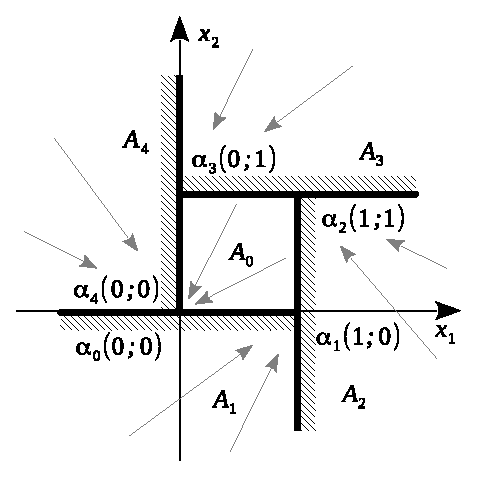
\includegraphics[width=0.4\linewidth]{quad3.eps}
	\caption{Разбиение плоскости, отмеченные точки и направления сдвигов}
	\label{fig:somelabel}
	%\vspace{2cm}
\end{figure}

Положим $E=E_0=\mathbb{R}^2$.
Разобьём $\mathbb{R}^2$ на пять непересекающихся связных множеств следующим образом:
$$
	A_0 = \{ (x_1, x_2) \mid 0 < x_1 < 1, 0 < x_2 < 1\},
$$
$$
	A_1 = \{ (x_1, x_2) \mid x_1 < 1, x_2 \leq 0  \},
	A_2 = \{ (x_1, x_2) \mid x_1 \geq 1, x_2 < 1  \},
$$
$$
	A_3 = \{ (x_1, x_2) \mid x_1 > 0, x_2 \geq 1  \},
	A_4 = \{ (x_1, x_2) \mid x_1 \leq 0, x_2 > 0  \}
$$
и отметим точки
$\alpha_1=(1, 0)$,
$\alpha_2=(1, 1)$,
$\alpha_3=(0, 1)$ и
$\alpha_4=\alpha_0=(0, 0)$
(двойное обозначение используется для удобства работы с индексами).

Сразу заметим, что $\alpha_i \in \overline{A_i}$, $i=0,...,4$ и
$\alpha_i \in A_{i+1}$, $i=0,...,3$ (тогда как $\alpha_4 = \alpha_0 \in A_{1}$).

Таким образом, вся координатная плоскость оказалась разбита на четыре угла $A_1, ..., A_4$ и квадрат $A_0$.
Квадрат не включает свои границы; для каждого угла одна его сторона включается в угол,
а вторая сторона и вершина --- нет (они включаются в <<соседний>>).
Именно за счёт такого разбиения и достигается эффект примера.

В дальнейшим первый нижний индекс (в случае, когда нижних индексов два)
будет отвечать за номер области и обозначаться через $i$,
$i=0, ..., 3$, второй --- за координату и обозначаться $j$, $j=1, 2$.

Рассмотрим дифференциальное уравнение
\begin{equation}\label{difur_primer_R2}
	\frac{dx_j(t)}{dt} = -\gamma_{ij}(x_j(t)-p_{ij})^2,
\end{equation}
где
$
	\gamma_{ij} = \operatorname{sgn}(x_j(0)-p_{ij}), j=1,2;
	(x_1, x_2) \in A_i,  \alpha_i = (p_{i1},p_{i2}).
$

Де-факто это --- система из двух дифференциальных уравнений, по одному уравнению на координату.
Обратим внимание, что каждая координата меняется независимо от другой и гиперболически стремится
к некоторому предельному значению (это будет показано далее).

Для удобства решения представим это уравнение в виде
\begin{equation*}
	\frac{d(x_j(t) - p_{ij})}{dt} = -\gamma_{ij}(x_j(t)-p_{ij})^2,
\end{equation*}
т.е. добавим константу под знаком дифференциала.

Если $\gamma_{ij} = 0$, то $x_j(t) \equiv const$.
Если $\gamma_{ij} \neq 0$, то разделим переменные $t$ и $(x_j(t) - p_{ij})$:
\begin{equation*}
	\frac{d(x_j(t) - p_{ij})}{-\gamma_{ij}(x_j(t)-p_{ij})^2} = dt ,
\end{equation*}
откуда
\begin{equation*}
	\frac{\gamma_{ij}}{x_j(t)-p_{ij}} = t+C_0, C_0 > 0
\end{equation*}
(неравенство на $C_0$ налагается для обеспечения существования решения на всей положительной полуоси),
или, что то же самое,
\begin{equation}\label{primer_R2_x_j}
	x_j(t) = \frac{\gamma_{ij}}{t+C_0}+p_{ij}, C_0 > 0
\end{equation}
откуда
\begin{equation*}
	x_j(t) \xrightarrow[t\to \infty ]{}{p_{ij}},
\end{equation*}
при этом знак разности $x_j(t) - p_{ij}$ не меняется.
Заметим, что формула (\ref{primer_R2_x_j}) верна и для случая $\gamma_{ij}=0, x_j(0)=p_{ij}$.

Выпишем теперь оператор сдвига.
Положим в (\ref{primer_R2_x_j}) $t=0$, получим
$$
	x_j(0) = \frac{\gamma_{ij}}{C_0}+p_{ij}
$$

Выразив отсюда $C_0$, подставим полученное выражение и выражение для $\gamma_{ij}$ в (\ref{primer_R2_x_j}).
Таким образом, оператор сдвига по траекториям уравнения (\ref{difur_primer_R2}) имеет вид
\begin{equation}\label{primer_R2_oper_sdviga}
	\tilde{S}_t(x_{j}(0)) = \frac{x_{j}(0)-p_{ij}}{|x_{j}(0)-p_{ij}|t+1}+p_{ij}
\end{equation}

Заметим, что числитель дроби не зависит от $t$, а знаменатель всегда строго положителен.
Следовательно, разность $\tilde{S}_t(x_j(0)) - p_{ij}$ сохраняет знак,
и траектория, начавшись в области $A_i$, никогда не перейдёт в другую область $A_{i'}$, $i \neq i'$.

Для примера рассмотрим точку $B(0; -1) \in A_1$.
По построению $\alpha_1 = (p_{11}; p_{12}) = (1; 0)$, т.~е. $p_{11} = 1$, $p_{12} = 0$.
Соотвествующие операторы сдвига для координат точки $B$ имеют вид:
$$
	\tilde{S}_t(x_{1}(0))
	= \frac{x_{1}(0)-p_{11}}{|x_{1}(0)-p_{11}|t+1}+p_{11}
$$
$$
	\tilde{S}_t(x_{2}(0))
	= \frac{x_{2}(0)-p_{12}}{|x_{2}(0)-p_{12}|t+1}+p_{12},
$$
т.~е.
$$
	\tilde{S}_t(0)
	= \frac{0-1}{|0-1|t+1}+1
	= \frac{-1}{t+1}+1
	= 1 - \frac{1}{t+1}
	< 1
$$
$$
	\tilde{S}_t(-1)
	= \frac{-1-0}{|-1-0|t+1}+0
	= \frac{-1}{t+1}+0
	= -\frac{1}{t+1}
	< 0
$$
Мы видим, что рассматриваемая траектория действительно не выходит за пределы угла $A_1$.


Для $x_0 \in A_i$ имеем
\begin{equation}\label{primer_R2_stremlenie}
	S_t(x_0) \xrightarrow[t \to \infty]{} \alpha_{i},
\end{equation}
причём монотонно по $t$.
Действительно,
\begin{multline}
	\|S_t(x_0) - \alpha_i\| \leq
	\sqrt{2} \max_{j=1,2} \left| \frac{x_{j}(0)-p_{ij}}{|x_{j}(0)-p_{ij}|t+1} + p_{ij} - p_{ij}  \right| =
	\sqrt{2} \max_{j=1,2} \left| \frac{x_{j}(0)-p_{ij}}{|x_{j}(0)-p_{ij}|t+1} \right| \leq
	\\ \leq
	\sqrt{2} \max_{j=1,2} \left| \frac{x_{j}(0)-p_{ij}}{|x_{j}(0)-p_{ij}|t} \right| =
	\sqrt{2} \max_{j=1,2} \left| \frac{1}{t} \right| =
	\frac{\sqrt{2}}{t} \xrightarrow[t \to \infty]{} 0
\end{multline}

Заметим, что эта оценка равномерна по $x_{j}(0)$.
Более того, из того, что $\alpha_i \in A_{i+1}$, $i=0,...,3$,
следует, что $S_t(\alpha_i) \xrightarrow[t \to \infty]{} \alpha_{i+1}$,
т.е. множество функций-констант
$$
	U = \{ u_i(t) \equiv \alpha_i \}_{i=0}^{3}
$$
не пересекается со множеством решений уравнения (\ref{difur_primer_R2}).

Покажем теперь, что $U$ --- траекторный аттрактор в смысле [\cite{Zelenaya}, опред. 3.2.3].
Компактность и ограниченность множества из четырёх функций-констант в пространствах
$C(\mathbb{R}_+; \mathbb{R}^2)$ и $L_\infty(\mathbb{R}_+; \mathbb{R}^2)$ очевидна.
Очевидно и то, что $U$ трансляционно инвариантно.

Осталось показать, что $U$ есть притягивающее множество в пространстве траекторий $H^+$ уравнения (\ref{difur_primer_R2}).
Действительно, пусть $M>0$ и $B\subset H^+$ --- ограниченное в $L_\infty(\mathbb{R}_+; \mathbb{R}^2)$ множество.
Тогда
\begin{multline*}
	h_{C([0,M];\mathbb{R}^2)}(\Pi_M T(t)B,\Pi_M U) =
	\sup_{v\in B} \inf_{u\in U} \| T(t) v - u \|_{C([0,M];\mathbb{R}^2)} =
	\\ =
	\sup_{v\in B} \min_{i=0,..,3} \| T(t) v - u_i \|_{C([0,M];\mathbb{R}^2)} =
	\sup_{v\in B} \min_{i=0,..,3} \max_{s\in[0,M]} \| (T(t) v)(s) - u_i(s) \| =
	\\ =
	\sup_{v\in B} \min_{i=0,..,3} \max_{s\in[0,M]} \| (T(t) v)(s) - \alpha_i \| =
	\sup_{v\in B} \min_{i=0,..,3} \max_{s\in[t,t+M]} \| v(s) - \alpha_i \| \leq
	\frac{\sqrt{2}}{t} \xrightarrow[t\to + \infty]{} 0
\end{multline*}
Таким образом, $U$ --- действительно траекторный аттрактор, пересечение которого с пространством траекторий
уравнения (\ref{difur_primer_R2}) пусто.

\section{Аттрактор полугруппы трансляций (динамической системы)}

Покажем теперь, что $(\mathbb{R}^2,\mathbb{R}^2)$--аттрактора полугруппы трансляций в данном примере не существует.
Предположим противное, т.е. что существует $P$ --- аттрактор полугруппы трансляций,
порождаемой оператором сдвига (\ref{primer_R2_oper_sdviga}).

Пусть сначала $\exists(i=0,...,4)[\alpha_i \notin P]$.
Тогда в силу условия (а) из определения аттрактора полугруппы трансляций вытекает,
что $A$ --- компактно в $\mathbb{R}^2$.
Тогда расстояние $\rho$ от $P$ до $\alpha_i$ положительно.

Положим $\varepsilon = \frac{\rho}{3} > 0$ и покажем,
что условие притяжения из определения аттрактора полугруппы трансляций не выполняется.

Рассмотрим $V_\varepsilon = A_i \cap B(\alpha_i, \varepsilon)$ и некоторое решение $x_\varepsilon(t)$
такое, что $x_\varepsilon(0) \in V_\varepsilon$.
Тогда в силу монотонности стремления (\ref{primer_R2_stremlenie})
$\forall(t>0)[x_\varepsilon(t) \in V_\varepsilon]$.
Но $V_\varepsilon$ отделено от $P$, следовательно, $x_\varepsilon{t}$ не попадает в $\varepsilon$--окрестность $P$
ни при каких положительных $t$, что доказывает нарушение условия притяжения.

Значит, если аттрактор $P$ полугруппы трансляций существует, то $\alpha_i \in P, i=0,...,4$.
Но тогда $\forall(t>0)[S_t P \ne P]$.
Действительно, траектория, выходящая из $\alpha_i$, стремится к $\alpha_{i+1}$;
а все траектории, выходящие из точек области $A_i$, стремятся к $\alpha_i$,
но никогда не достигают её.

Следовательно, аттрактора полугруппы трансляций в данном случае не существует.
